\section{Introduction}

Nature-inspired optimization algorithms have been used successfully in the last
decades to tackle complex problems \cite{yang2014nature}. These
algorithms include evolutionary algorithms (EAs)
\cite{back1996evolutionary} and swarm intelligence (SI)
\cite{kennedy2006swarm}. % Maybe mention a few more, like bee o others
                         % like that? - JJ
Genetic Algorithms (GAs) 
\cite{holland1992adaptation,eiben2003genetic}, and
Differential Evolution (DE) \cite{karabouga2004simple} are two popular
EAs, while examples of SI algorithms 
\cite{kennedy2006swarm} are particle swarm optimization (PSO)
\cite{clerc2010particle}, and ant colony algorithms (ACO) \cite{dorigo1999ant}.
A common characteristic of these kind of methods is the
use of an initial set of random candidate solutions that are manipulated by the
algorithm to generate a new set of candidates, and because of this, we commonly
referred to them as population-based algorithms. % There are other
                                % population based algorithms that are
                                % not natural, such as PBIL. Maybe you
                                % could mention them - JJ

Since instead of piecewise constructing a population or changing it
incrementally, all members of the population have to be evaluated to
obtain a fitness or score that will be used to select them (or not), a
drawback of this kind of algorithms is that they can be computationally
expensive since it is difficult to overcome that $n$ factor, where $n$
is the population size, in the complexity of every iteration of the
algorithm. That is why researchers have been proposing some form of
parallelization since early on \cite{muhlenbein1988evolution} to
increase their scalability. % Not scalability, but wallclock timing - JJ
One of the first methods of parallelization was the island
model, which lead to an increased performance
\cite{gorges1990explicit,grosso1985computer}. The concept was to divide the
population into smaller populations that communicated with each other. Other
population-based algorithms have adopted the technique, and since then,
researchers have found additional advantages besides the execution speed, 
these include avoiding a premature convergence and maintaining the diversity of the
global population \cite{li2015multi}, we are going to call these methods 
multi-population algorithms \cite{Ma2019}. The relative 
isolation in which populations carry out the algorithm, together with the
synchronous or asynchronous communication, helps to increase the overall
diversity since each population will search in a particular area, at least
between communications. Multi-population algorithms use a form of
communication to recombine or migrate candidate solutions between populations
to avoid premature convergence, since smaller populations are known to perform
better for a given problem than bigger populations
\cite{li2016multi,wu2016differential}.  Even in some cases, a multi-population based
algorithm scales better due to these interactions, and the parallelism of the
operation \cite{ALBA20027}. 

Having many populations offers researchers many configuration options and
additional challenges when designing efficient multi-population algorithms.
Options include the number and size of populations, the interaction between
them, the search area of each population, and the search strategy and
parametrization of each population.  In this paper, we are interested in the
latter, that is, having multiple populations running with distinct parameters
and optimization algorithms. We can find in the literature, several
heterogeneous multi-population algorithms integrating variations of optimization
algorithms, and these often perform better than single-population or homogeneous
multi-population optimization algorithms\cite{wu2016differential,nseef2016adaptive}.
Heterogeneous algorithms add to
the problem of finding the correct parameter settings for each population;
because some parameters affect the accuracy of the solution and the convergence
speed of the individual algorithms as they tip the balance between exploration
and exploitation of the search space. On the other hand, current studies show
that by having a high number of populations communicating in parallel, the
effect of the individual parameters of each population is compensated by those
selected in other populations \cite{li2016multi,tanabe2013evaluation}. Some
level of heterogeneity can be implemented by just changing the configuration
parameters of each population, but in this case, we are interested in
heterogeneous search strategies.

Therefore, in this paper, we implemented an asynchronous multi-population
algorithm version, using a message queue for inter-process communication \cite{
guervos2018introducing}, and a reactive migration procedure, in which we compare
three heterogeneous configurations using a randomized parameter technique. We
experimented with all populations using a GA or PSO search strategies, versus an
ensemble multi-population with both GA and PSO algorithms, using as a benchmark,
the first five functions of the BBOB testbed. We compare the options by
measuring the average running time (aRT) as the number of functions (\#FEs), as
the objective is to prove that the advantage of heterogeneous configurations
resides not only in the increased scalability but also in the search
performance. 

The organization of the paper is as follows: First, Section \ref{soa} presents
state of the art relevant to our work. In Section \ref{method}, we present the
proposed method.  Section \ref{setup} describes the design of the empirical
evaluation we designed to assess the effectiveness of the method, and in Section
\ref{results}, we report and discuss the results. Finally, we offer the
conclusions of this paper and suggestions on future work in Section
\ref{conclusions}.


\section{State of the Art}
\label{soa}

\section{Proposed Method}
\label{method}

\section{Setup}
\label{setup}

\section{Results}
\label{results}

\begin{table}
    \small
    \caption{ DEAP GA EvoWorker Parameters }
    \label{tab:GAparams} 
    \centering
    \small
    \begin{tabular}{|l|c|}
      \hline
      Selection & Tournament size=12                            \\ \hline
      Mutation & Gaussian $\mu=0.0$, $\sigma=0.5$, indbp=0.05   \\ \hline
      Mutation Probability & [0.1,0.3]                          \\ \hline
      Crossover & Two Point                                     \\ \hline
      Crossover Probability  & [0.2,0.6]                          \\ \hline
    \end{tabular}
  \end{table}
  
  \begin{table}
    \small
    \caption{ EvoloPy PSO Parameters }
    \label{tab:PSOparams} 
    \centering
    \small
    \begin{tabular}{|l|c|}
      \hline
      $V_{max}$ & 6 \\ \hline
      $W_{max}$ & $0.9$ \\ \hline
      $W_{min}$ & $0.2$ \\ \hline
      $C_1$ & 2 \\ \hline
      $C_2$ & 2 \\ \hline
    \end{tabular}
  \end{table}


  \begin{table}
    \small
    \caption{Parameters used in the experiments with ten populations
    }
    \label{tab:params:10}
    \vspace{0.25cm}
    \centering
    \small
    \begin{tabular}{|l|c|c|c|c|c|c|}
      \hline
      Dimension        & 2  & 3  & 5  & 10 & 20  & 40  \\ \hline
      Generations      & 40 & 25 & 28 & 50 & 66  & 80  \\ \hline
      Population Size  & 50 & 60 & 60 & 70 & 100 & 125 \\ \hline
      Populations      & 10 & 10 & 10 & 10 & 10  & 10  \\ \hline
      Iterations       & 10 & 20 & 30 & 30 & 30  & 40  \\ \hline  
    \end{tabular}
\end{table}

% \begin{table*}
%   \caption{Some Typical Commands}
%   \label{tab:commands}
%   \begin{tabular}{ccl}
%     \toprule
%     Command &A Number & Comments\\
%     \midrule
%     \texttt{{\char'134}author} & 100& Author \\
%     \texttt{{\char'134}table}& 300 & For tables\\
%     \texttt{{\char'134}table*}& 400& For wider tables\\
%     \bottomrule
%   \end{tabular}
% \end{table*}
% % end the environment with {table*}, NOTE not {table}!


% %\begin{figure}
% %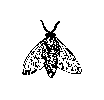
\includegraphics[height=1in, width=1in]{fly}
% %\caption{A sample black and white graphic
% %that has been resized with the \texttt{includegraphics} command.}
% %\end{figure}


% As was the case with tables, you may want a figure that spans two
% columns.  To do this, and still to ensure proper ``floating''
% placement of tables, use the environment \textbf{figure*} to enclose
% the figure and its caption.  And don't forget to end the environment
% with \textbf{figure*}, not \textbf{figure}!

% %\begin{figure*}
% %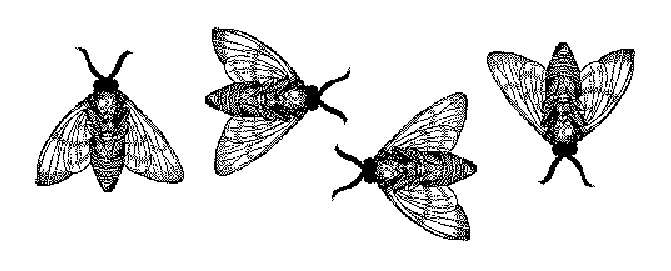
\includegraphics{flies}
% %\caption{A sample black and white graphic
% %that needs to span two columns of text.}
% %\end{figure*}


% %\begin{figure}
% %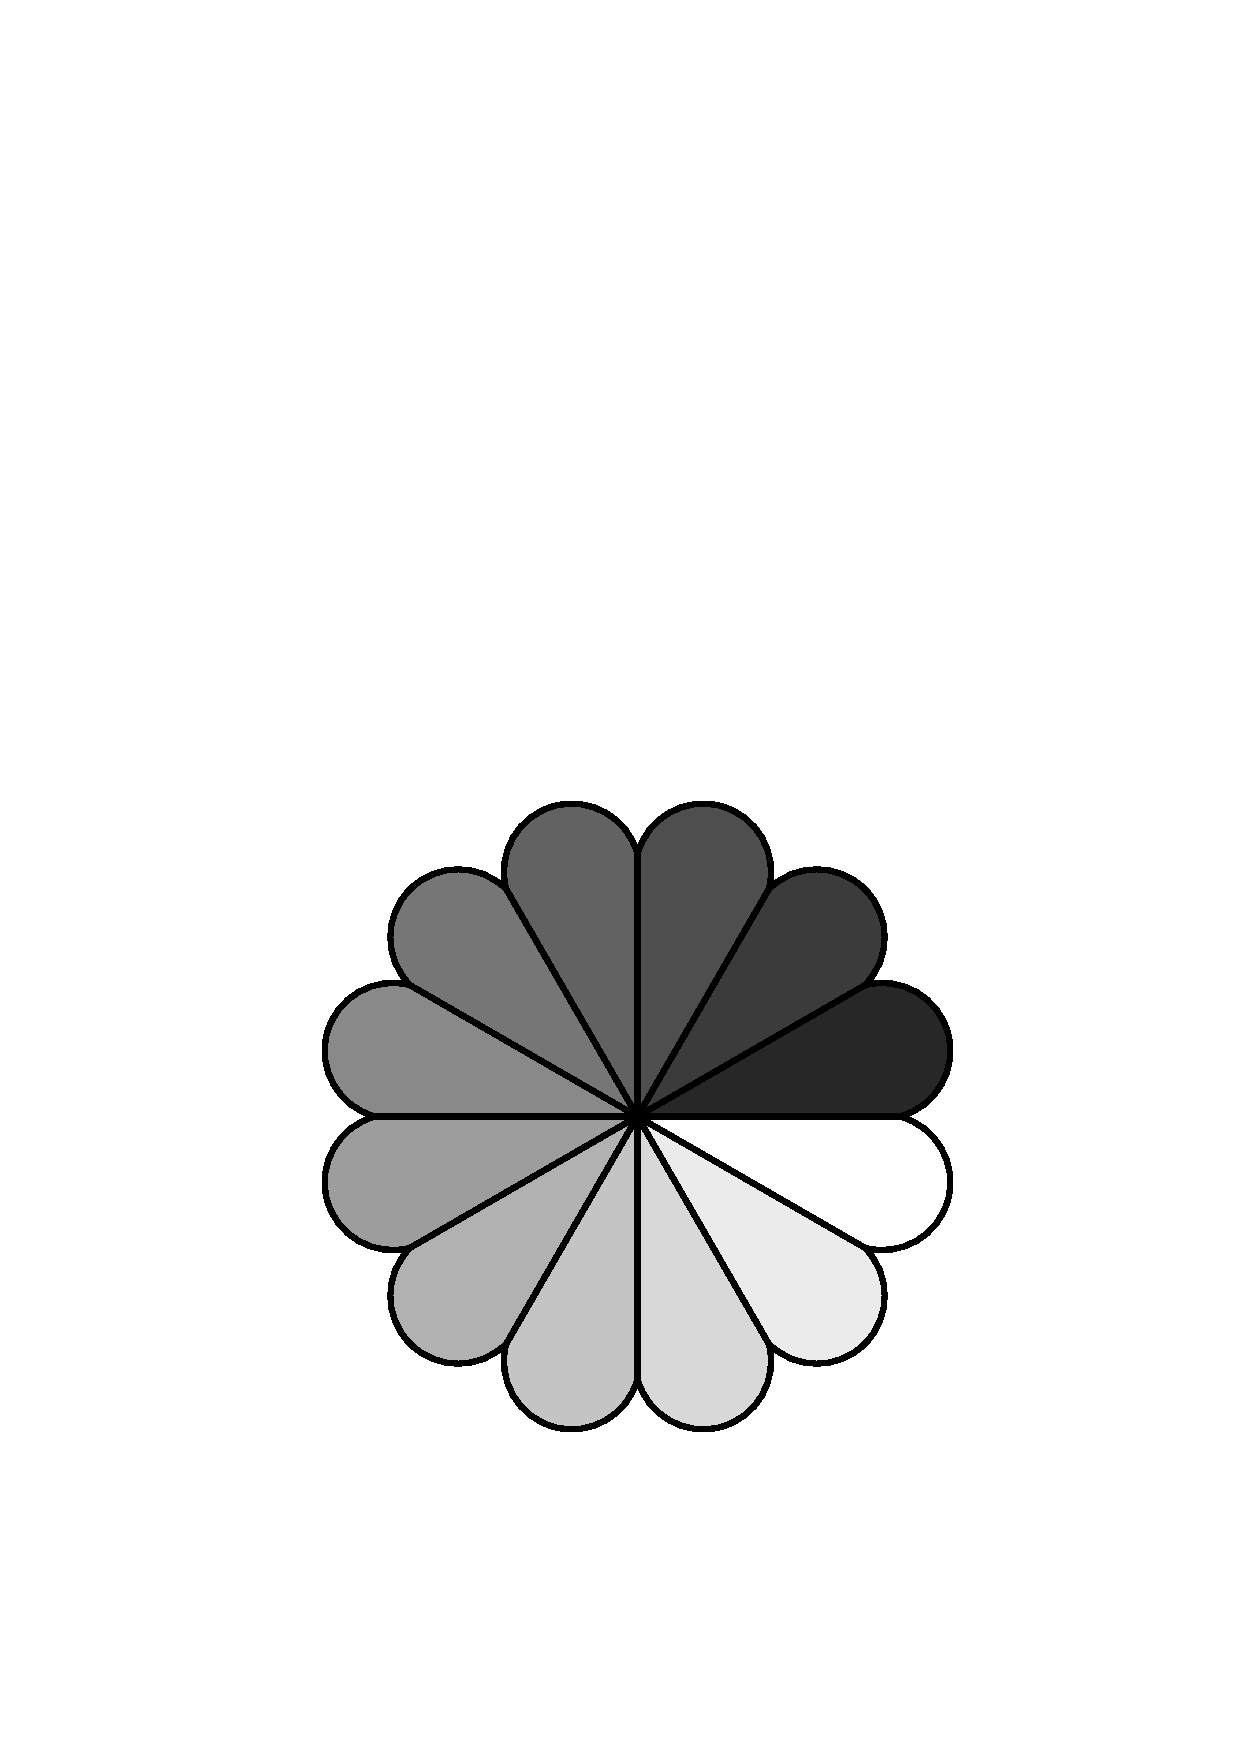
\includegraphics[height=1in, width=1in]{rosette}
% %\caption{A sample black and white graphic that has
% %been resized with the \texttt{includegraphics} command.}
% %\end{figure}

% \subsection{Experiment}
% \label{sec:exp_results}
% Having a multi-population based algorithm can decrease the execution time
% because of the parallel execution of the evolution. But, having heterogeneous 
% populations might enhance evolutionary search and needless
% evaluations than homogeneous systems; heterogeneous settings, if
% done right, increases the diversity of the whole population
% \cite{araujo2008multikulti}.

% But this is a rule of thumb, and it will depend on the degree of heterogeneity,
% as well as on the algorithm itself. Some level of heterogeneity can be
% implemented by just changing the configuration parameters of each population,
% but in this case, we are interested in a heterogeneous search strategy. 
% Therefore, in this experiment we compare a multi-population with only GA and PSO populations,
% versus an ensemble of GA and PSO algorithms. We tested on the first five functions of the
% BBOB testbed. We used ten populations and eight workers for the experiment and the
% same parameters as before.  


% \begin{figure*}[h!tb]
%     \begin{tabular}
%         {c@{\hspace*{-0.00001\textwidth}}
%          c@{\hspace*{-0.00001\textwidth}}
%          c@{\hspace*{-0.00001\textwidth}}
%         }
%     GA  &  PSO & GA \& PSO\\   
%     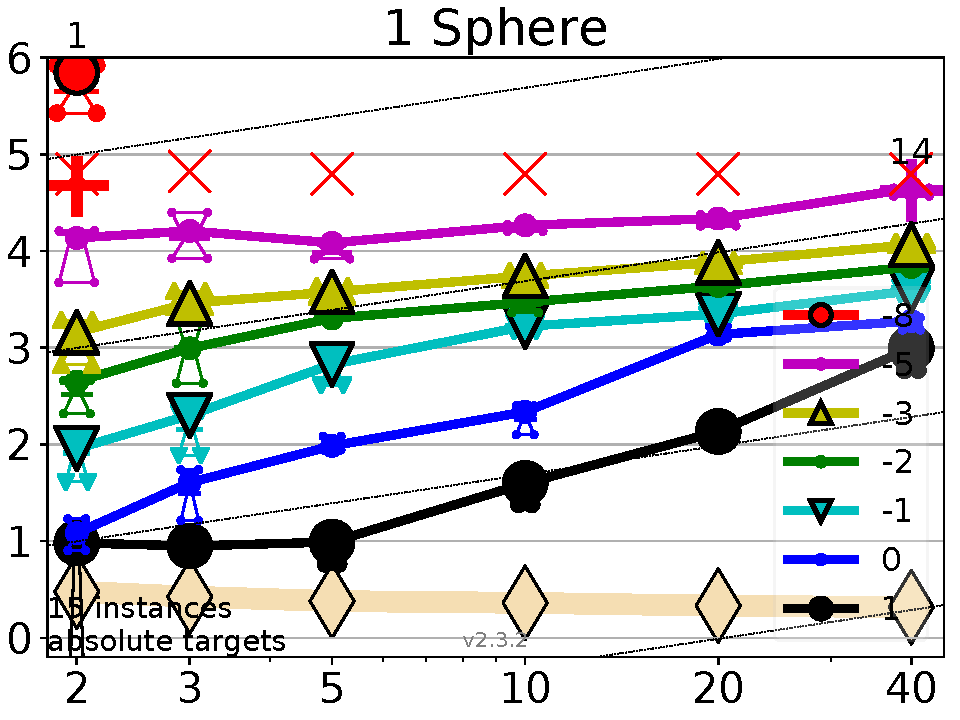
\includegraphics[width=0.28\textwidth]{GAOnly_f001}&
%     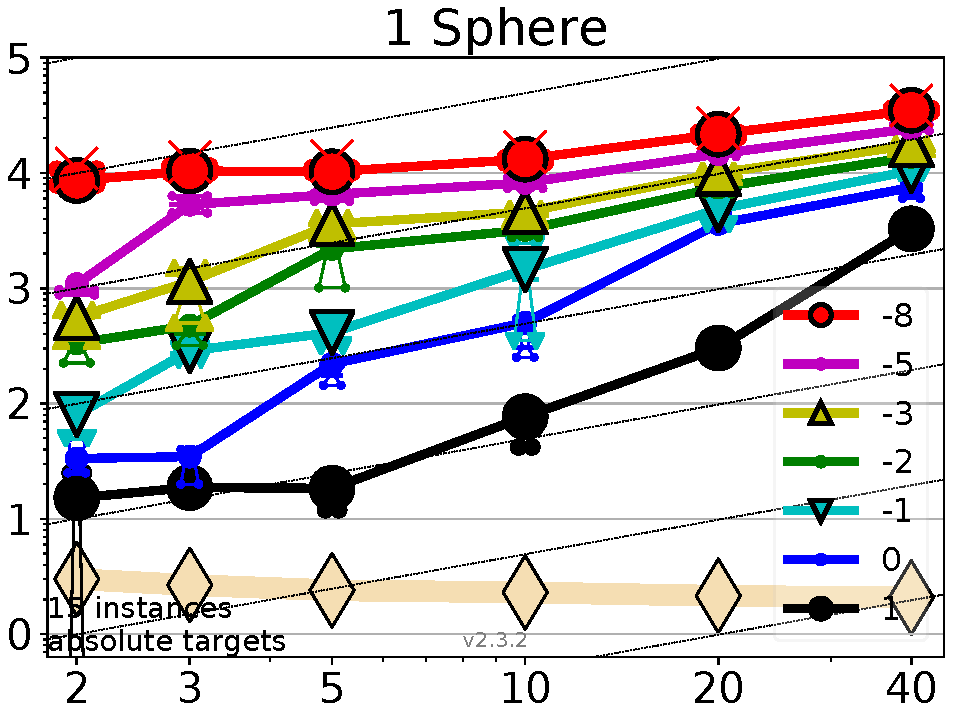
\includegraphics[width=0.28\textwidth]{PSOOnly_f001}&
%     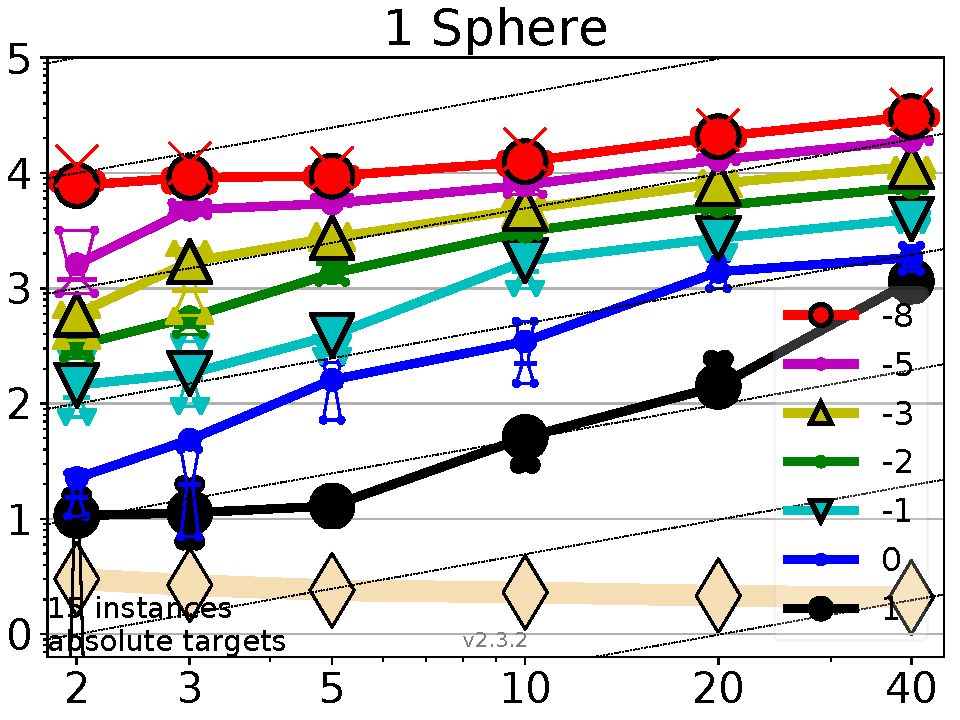
\includegraphics[width=0.28\textwidth]{GAPSO_f001}\\

%     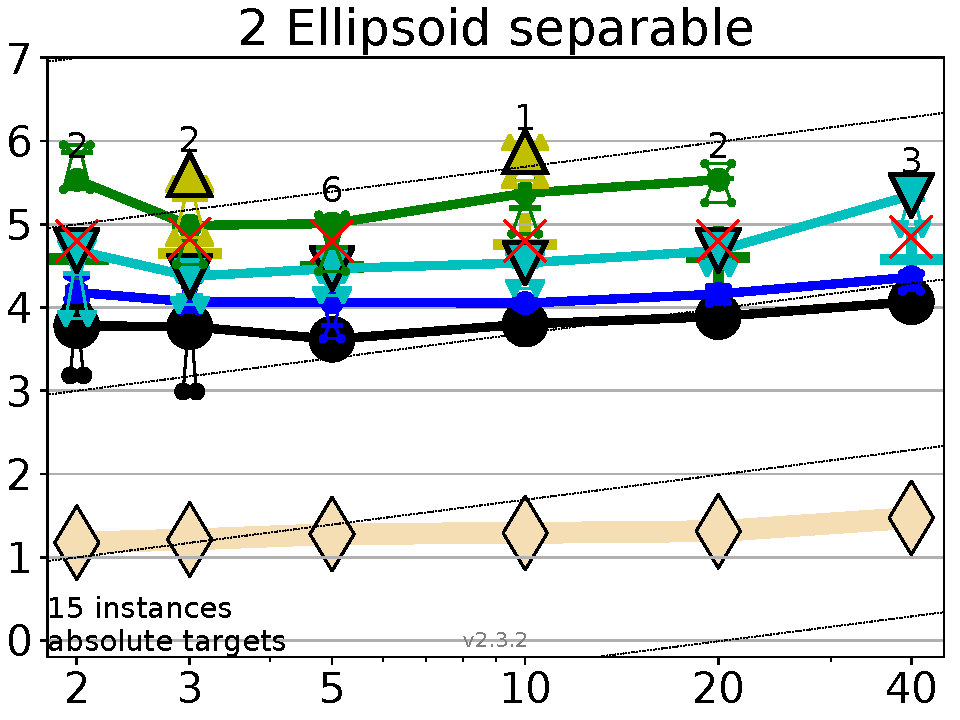
\includegraphics[width=0.28\textwidth]{GAOnly_f002}&
%     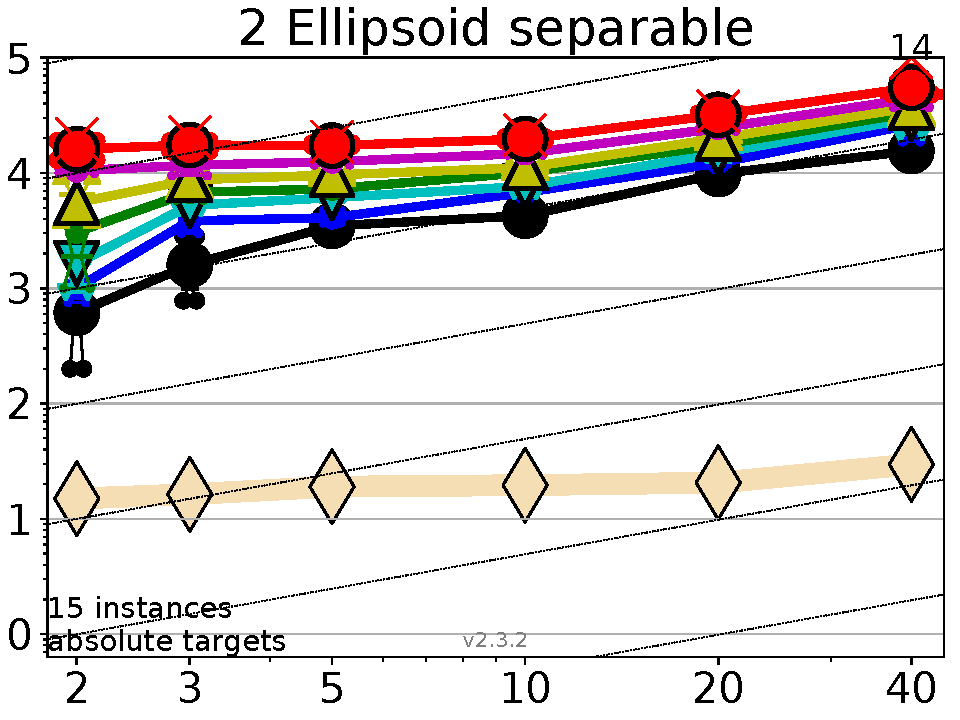
\includegraphics[width=0.28\textwidth]{PSOOnly_f002}&
%     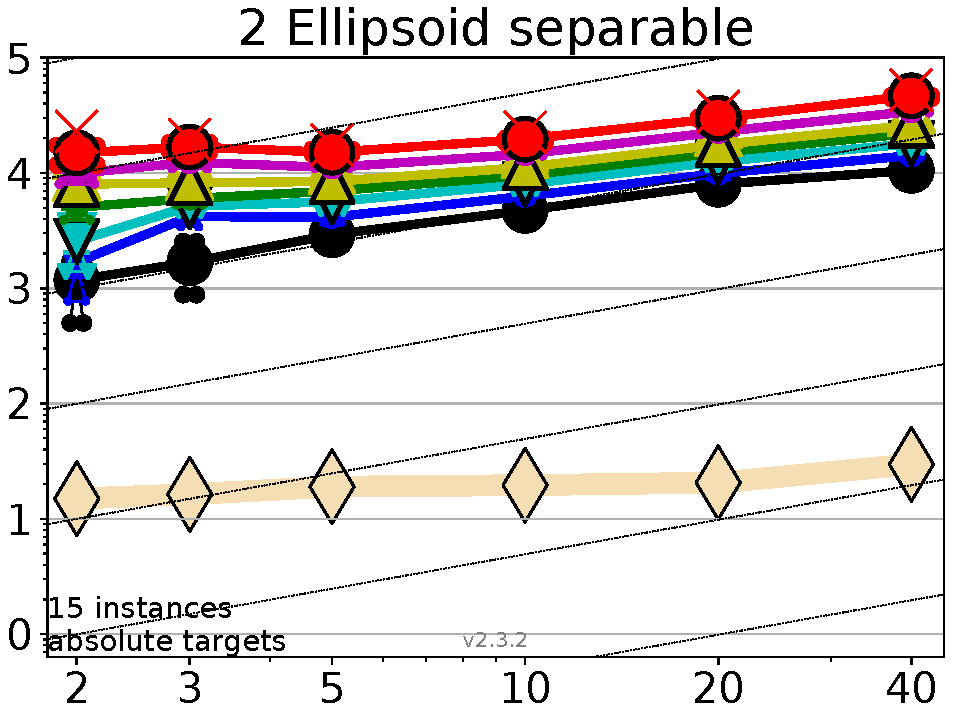
\includegraphics[width=0.28\textwidth]{GAPSO_f002}\\

%     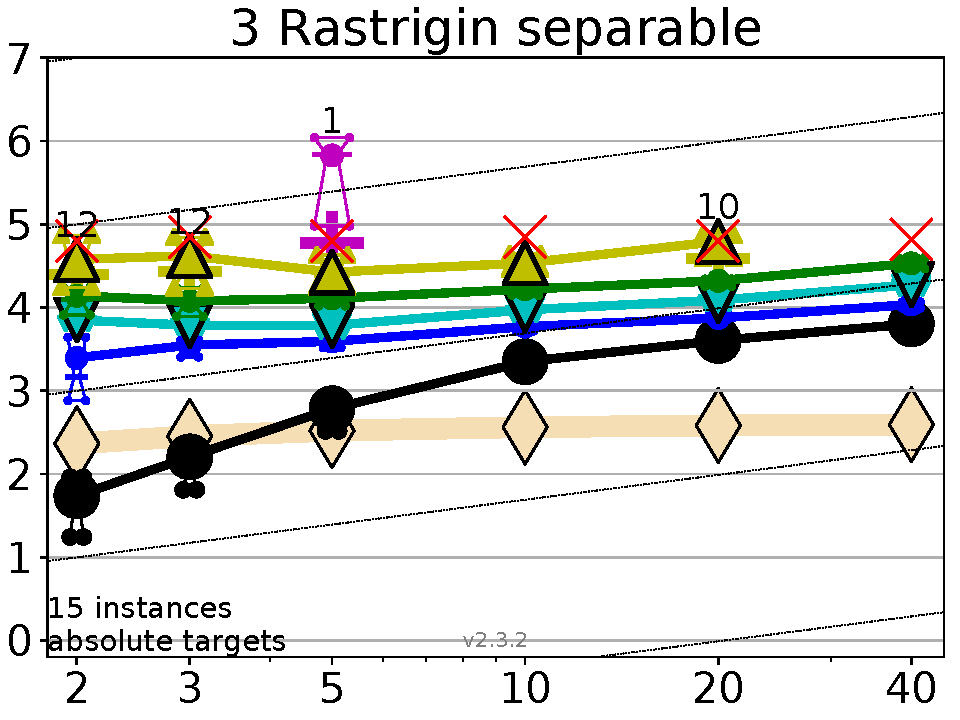
\includegraphics[width=0.28\textwidth]{GAOnly_f003}&
%     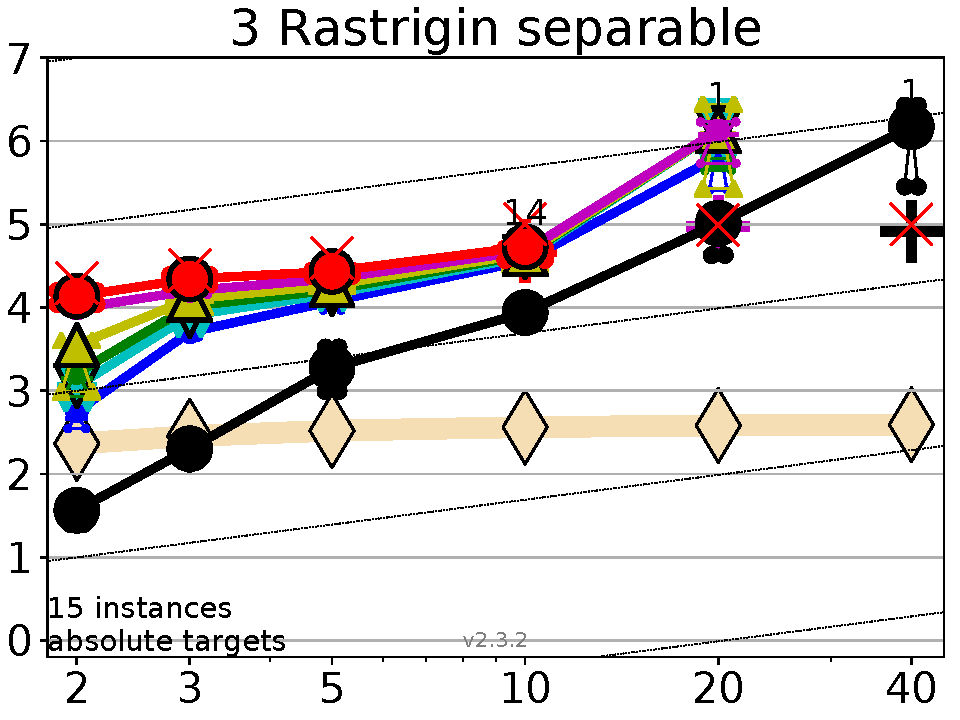
\includegraphics[width=0.28\textwidth]{PSOOnly_f003}&
%     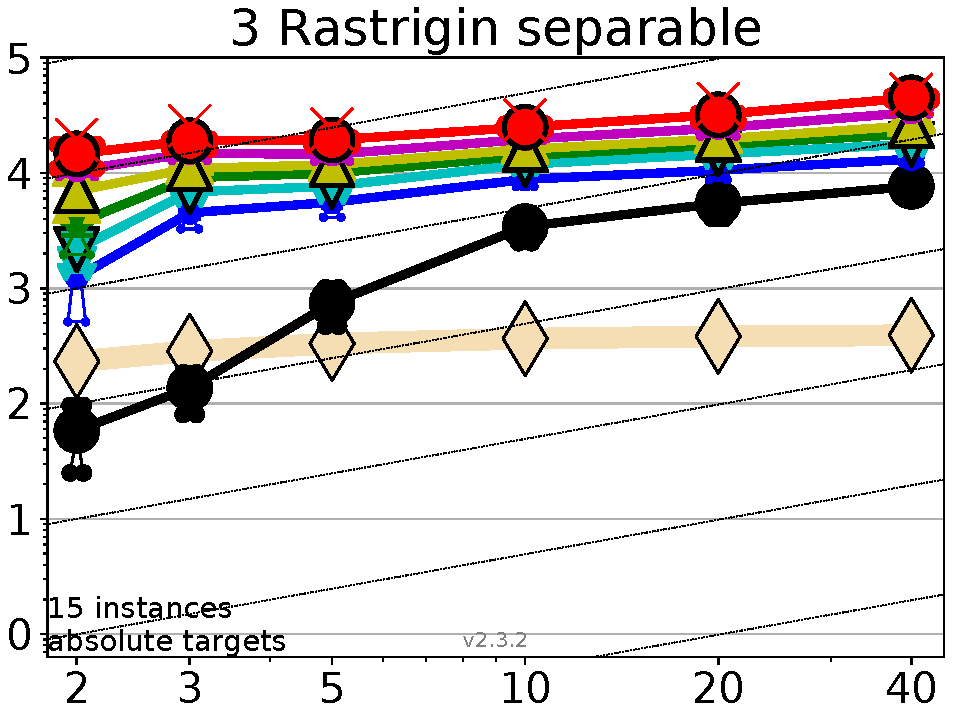
\includegraphics[width=0.28\textwidth]{GAPSO_f003}\\

%     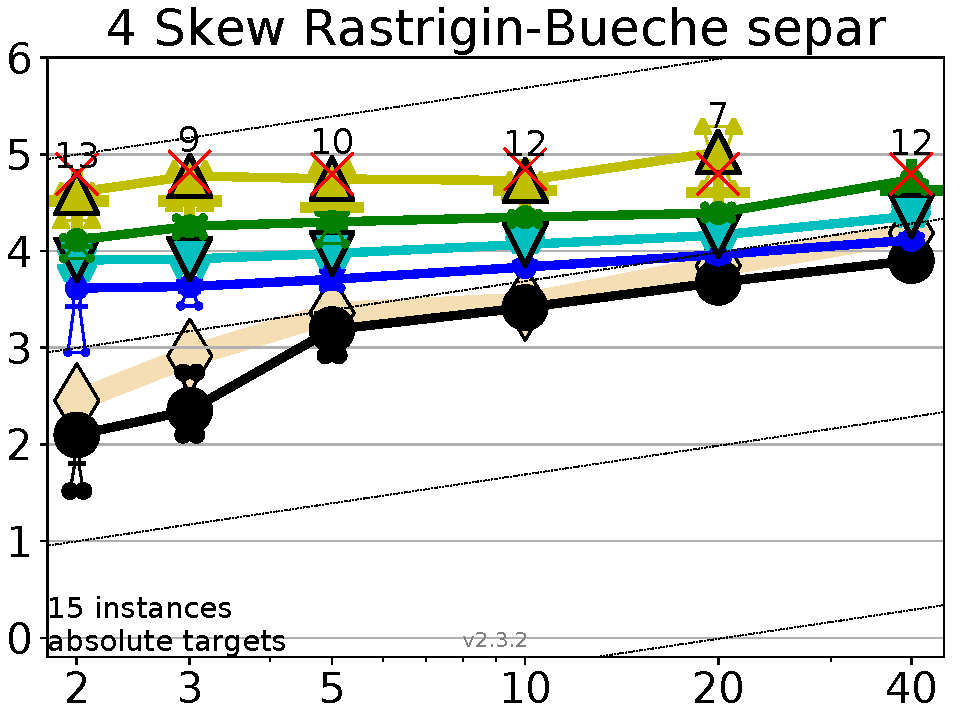
\includegraphics[width=0.28\textwidth]{GAOnly_f004}&
%     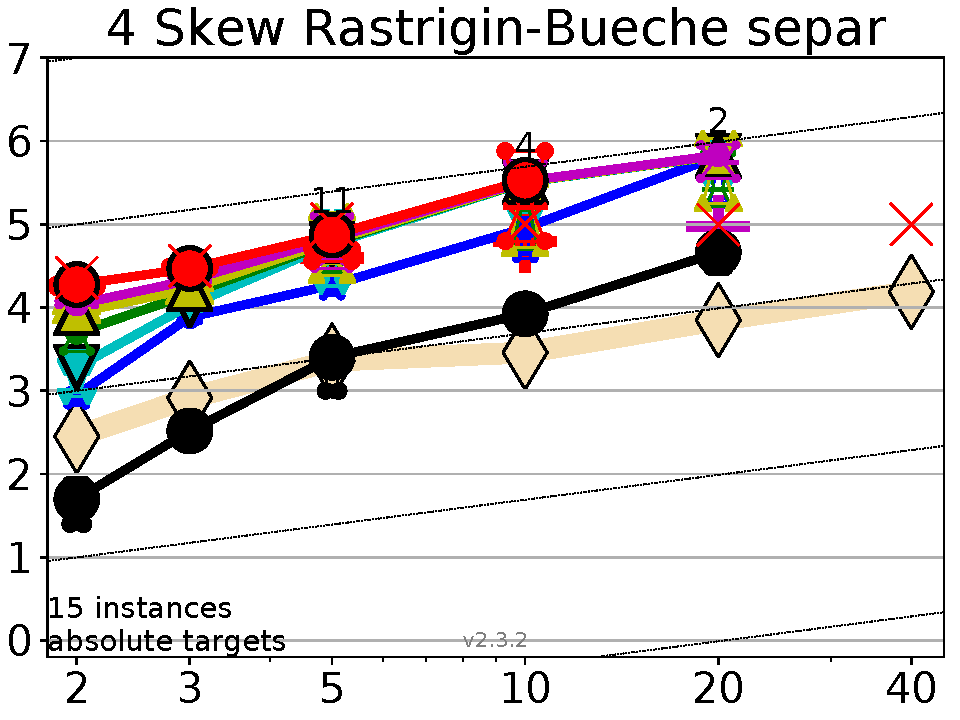
\includegraphics[width=0.28\textwidth]{PSOOnly_f004}&
%     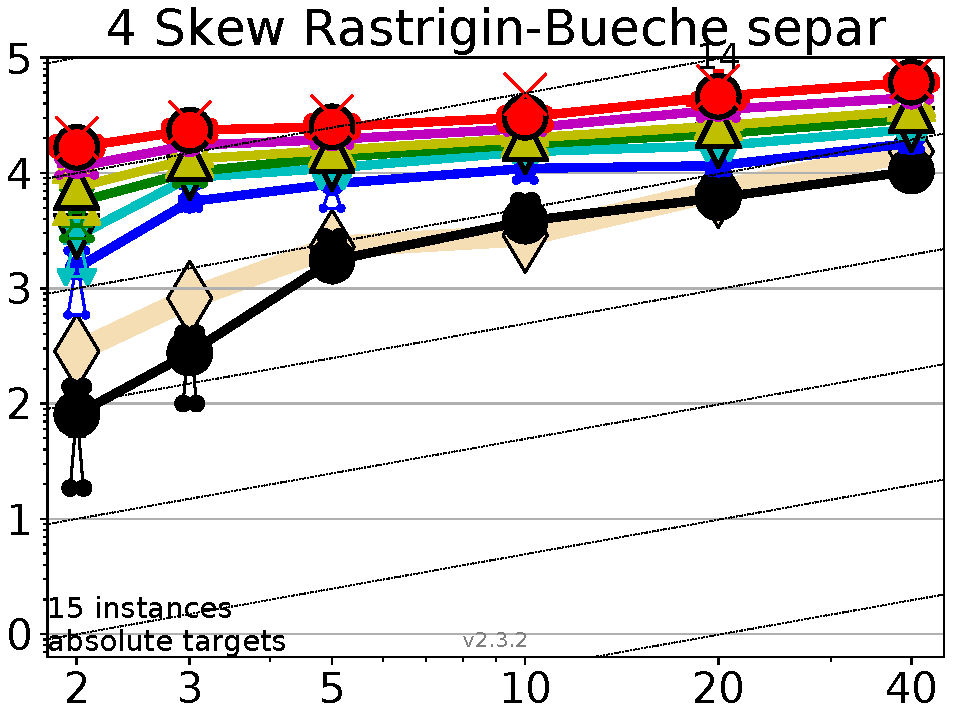
\includegraphics[width=0.28\textwidth]{GAPSO_f004}\\

%     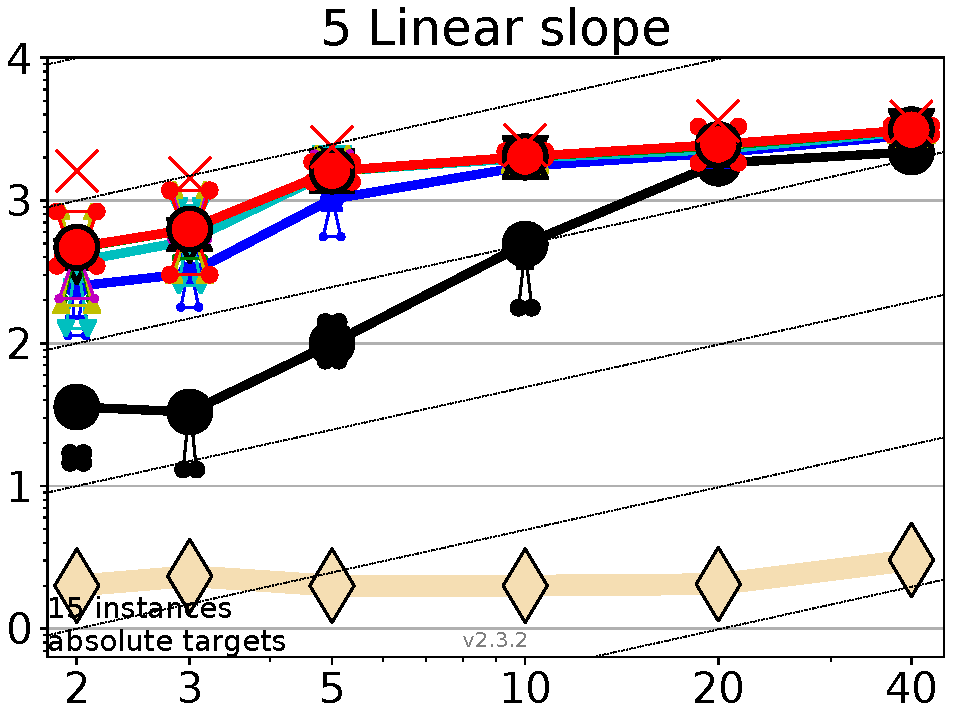
\includegraphics[width=0.28\textwidth]{GAOnly_f005}&
%     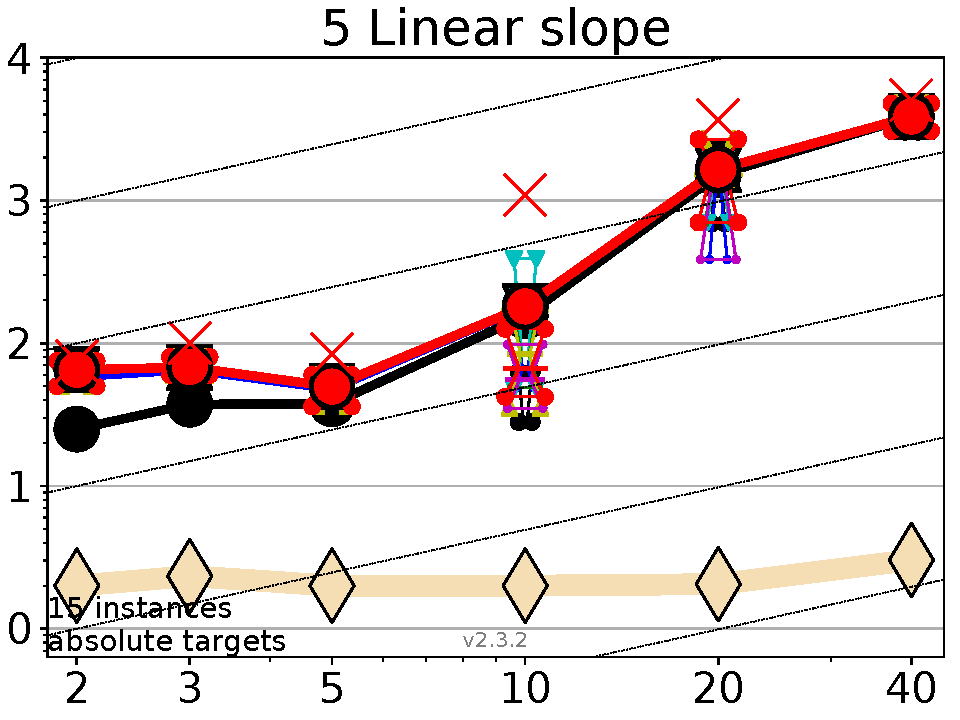
\includegraphics[width=0.28\textwidth]{PSOOnly_f005}&
%     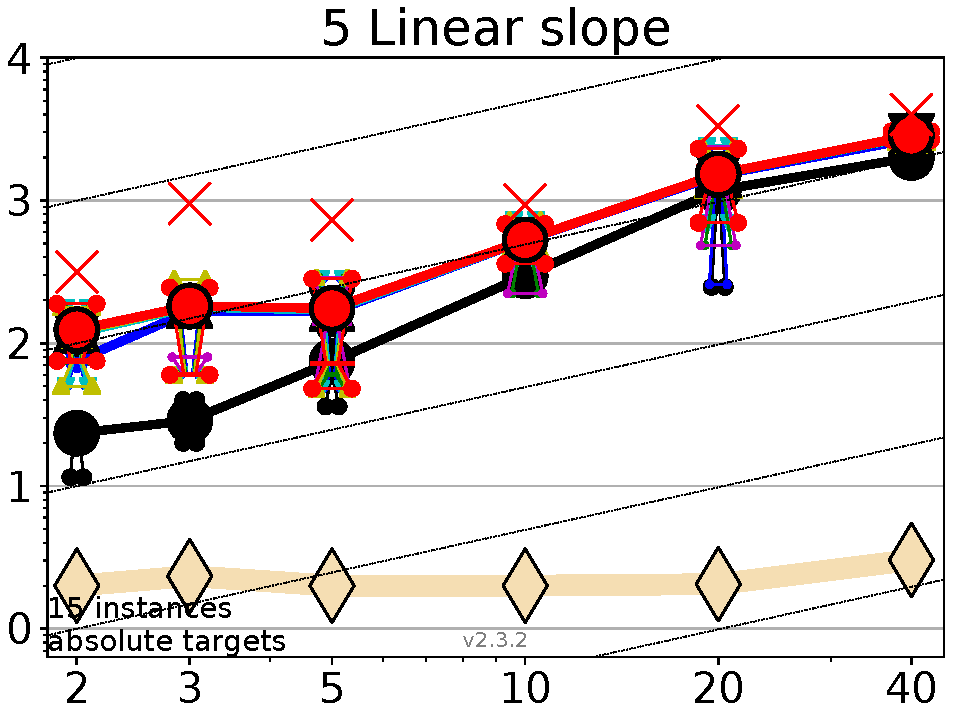
\includegraphics[width=0.28\textwidth]{GAPSO_f005}\\
%     \end{tabular}
%     \vspace{-3ex}
%      \caption{
%  Scaling of runtime with dimension to reach certain target values $\Delta f$. Lines:
%  average runtime (aRT); Cross ($+$): median runtime of successful runs to reach
%  the most difficult target that was reached at least once (but not always);
%  Cross (\textcolor{red}{$\times$}): maximum number of f-evaluations in any trial. Notched boxes:
%  interquartile range with median of simulated runs; All values are divided by
%  dimension and plotted as $log_{10}$ values versus dimension. 
%  %Shown is the aRT for
%  %fixed values of $\Delta f = 10k$ with $k$ given in the legend. 
%  Numbers above aRT-symbols
%  (if appearing) indicate the number of trials reaching the respective target.
%  %The light thick line with diamonds indicates the best algorithm from BBOB 2009
%  %for the most difficult target. Horizontal lines mean linear scaling, slanted
%  %grid lines depict quadratic scaling.
%  }
% \end{figure*}


    \begin{figure}[h!tb]
        \begin{tabular}
            {c@{\hspace*{-0.00001\textwidth}}
            % c@{\hspace*{-0.00001\textwidth}}
            }
           
        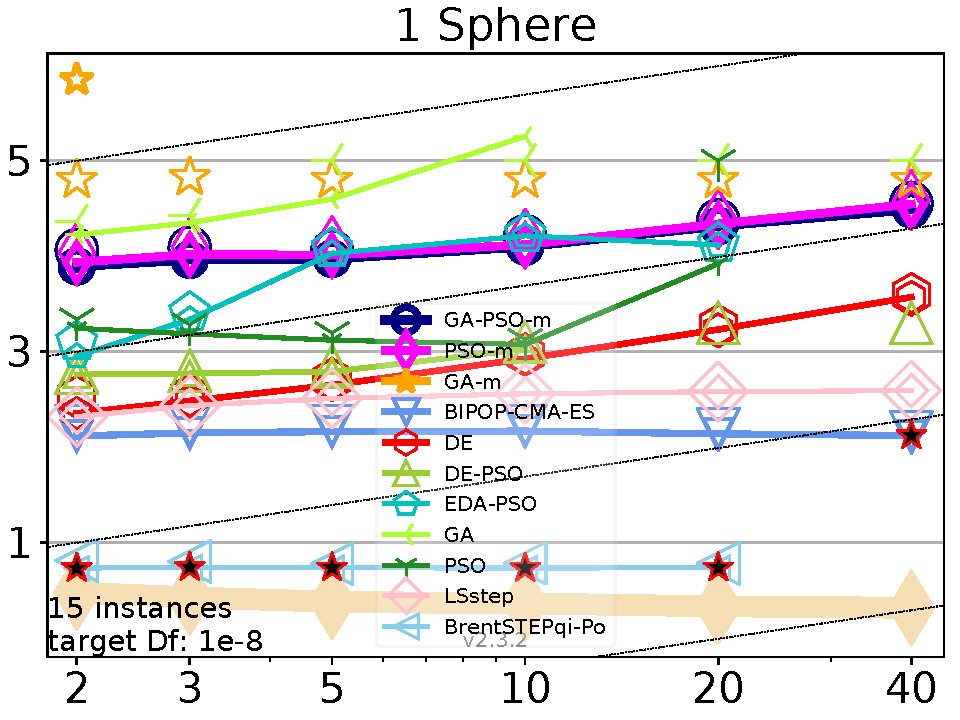
\includegraphics[width=0.28\textwidth]{ppfigs_f001}\\
        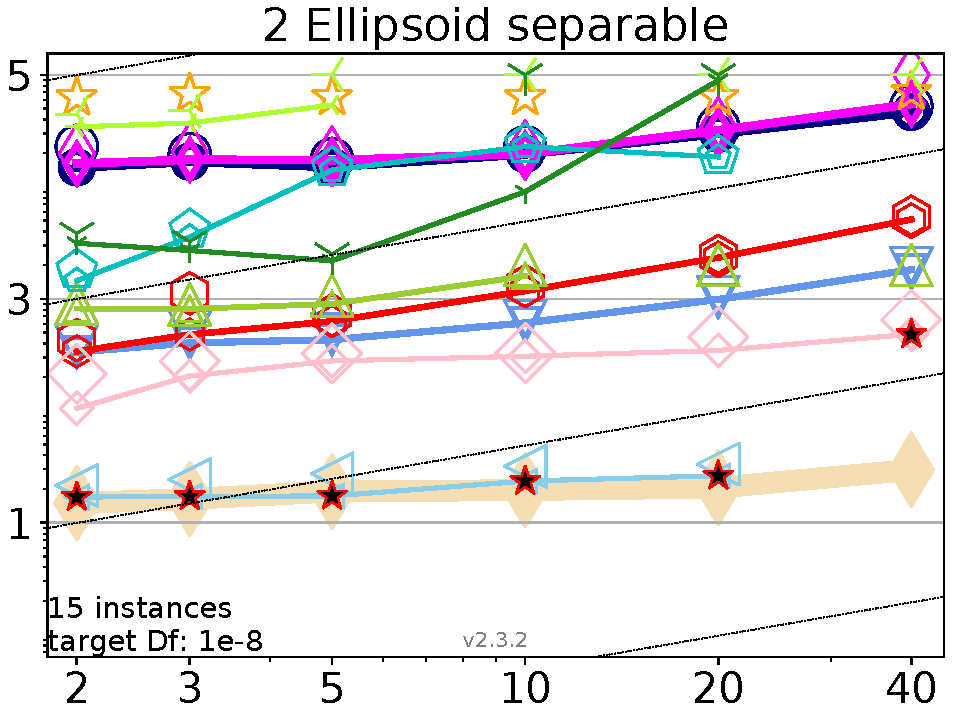
\includegraphics[width=0.28\textwidth]{ppfigs_f002}\\

        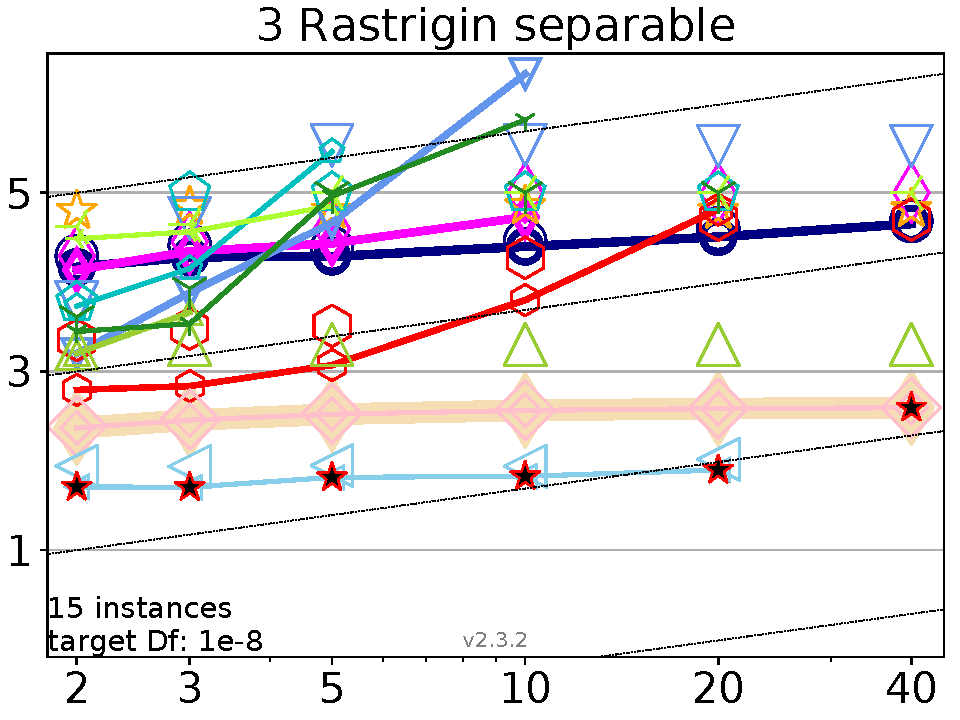
\includegraphics[width=0.28\textwidth]{ppfigs_f003}\\
        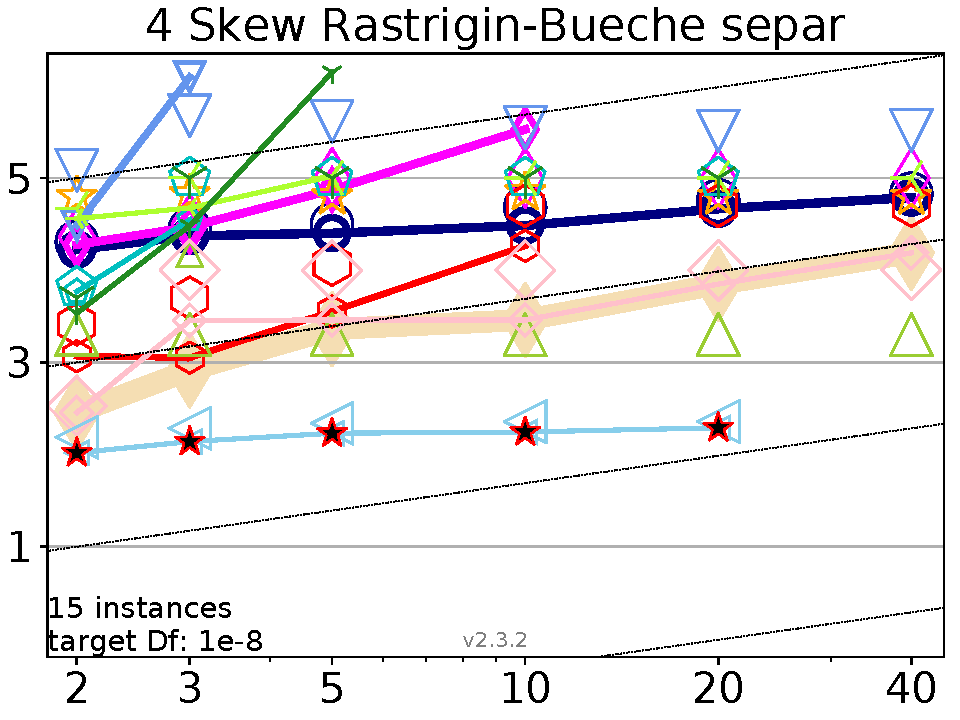
\includegraphics[width=0.28\textwidth]{ppfigs_f004}\\
        
        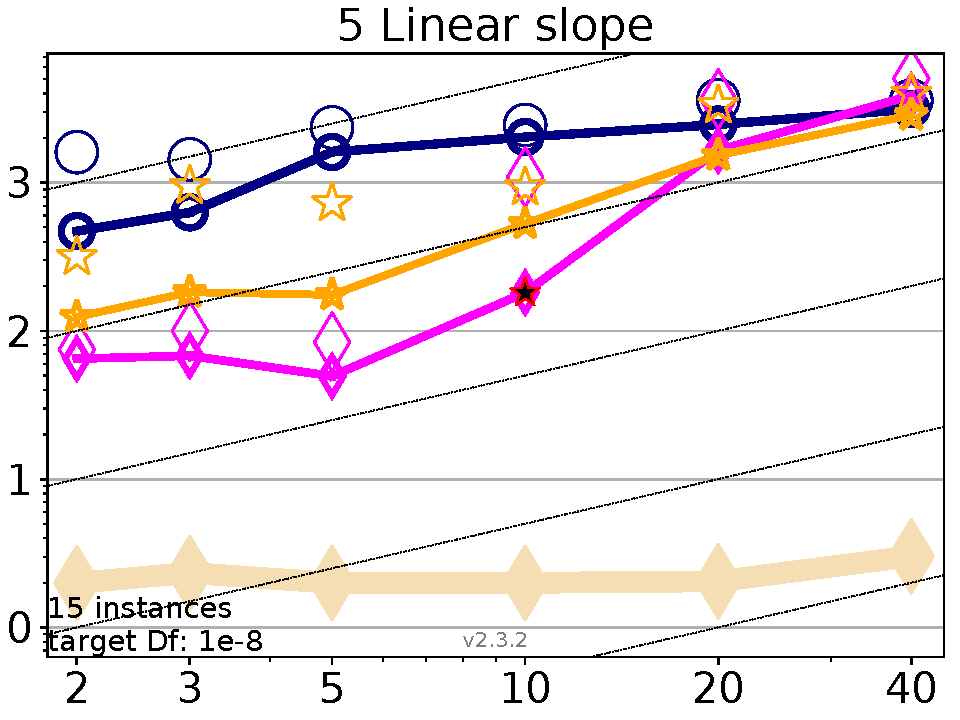
\includegraphics[width=0.28\textwidth]{ppfigs_f005}\\
        \end{tabular}
        \vspace{-3ex}
         \caption{Average running time (in \#FEs as $log_{10}$ value),
          divided by dimension for target function value $10^{-8}$ vs dimension. 
          Algorithms legends are given in $f_1$. Light symbols give the maximum number of 
          function evaluations from the longest trial divided by dimension. 
          Black stars indicate a statistically better result compared to 
          all other algorithms ($p < 0.01$) and Bonferroni 
          correction number of dimensions (six).}
    \end{figure}  

\section{Conclusions}
\label{conclusions}

\begin{acks}

  The authors would also like to thank the anonymous referees for
  their valuable comments and helpful suggestions. The work is
  supported by the 
\end{acks}
